На рисунке \ref{fig:timemodel} представлены результаты временного моделирования. На временной диаграмме продемонстрирована нормальная работа устройства: включение, работа, чтение режима, выключение, включение с другим адресом и т.д. Продемонстрированы разные режимы работы и переключения между ними. \\
Стоит отметить, что на временно диаграмме присутствуют риски: это вызвано некоторым запаздыванием в срабатывании элементов и на правильную работу устройства не влияет.
\begin{figure}
  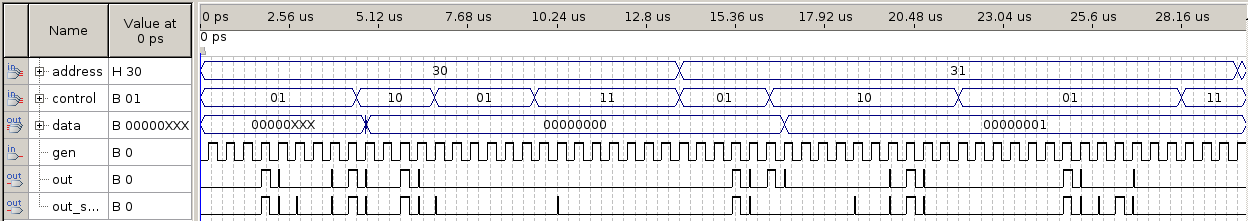
\includegraphics[scale=0.50]{./timing-two-modes.png}
  \caption{Временное моделирование узла.}
  \label{fig:timemodel}
\end{figure}